A base de dados de expressões faciais utilizada para o desenvolvimento deste trabalho é denominada \emph{Facial Expression Recognition Challenge} (FER2013). Esta base contém $35.887$ imagens faciais em escala de cinza com dimensões de $48\times 48$ pixels, rotuladas de maneira supervisionada segundo uma das sete expressões faciais universais, conforme amostras ilustradas na Figura \ref{fig:samples}.

\begin{figure}[!htb]
    \centering
    \caption{Amostras de imagens faciais da base de dados FER2013.}
    \label{fig:samples}
    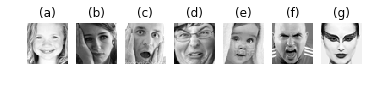
\includegraphics{images/samples.png}
    \floatfoot{(a)Felicidade, (b)Tristeza, (c)Medo, (d)Nojo, (e)Surpresa, (f)Raiva, (g)Neutro.}
\end{figure}

Conforme ilustra a Figura \ref{fig:samples}, é interessante notar algumas características particulares das imagens do FER2013 que ressaltam a relevância desta base de dados. Observa-se que, embora as faces estejam centralizadas nas imagens, elementos como cortes de cabelo, barba, óculos e até mesmo mãos encontram-se presentes, diminuindo a distância entre os exemplos contidos nesta base de dados e aqueles passíveis de ocorrência em um cenário realístico.

Os exemplos disponíveis na FER2013 se distribuem de maneira heterogênea perante as classes consideradas, conforme ilustra o gráfico da Figura \ref{fig:dataset}. O número de exemplos rotulado com a expressão ``nojo'', por exemplo, representam apenas $1.5\%$ do total de exemplos disponíveis. Estas características evidenciam o desbalanceamento do conjunto de dados considerado no tocante à quantidade de amostras por classe.

\begin{figure}[!htb]
    \centering
    \caption{Histograma da distribuição de imagens por tipo de expressão facial na base FER2013.}  \label{fig:dataset}
    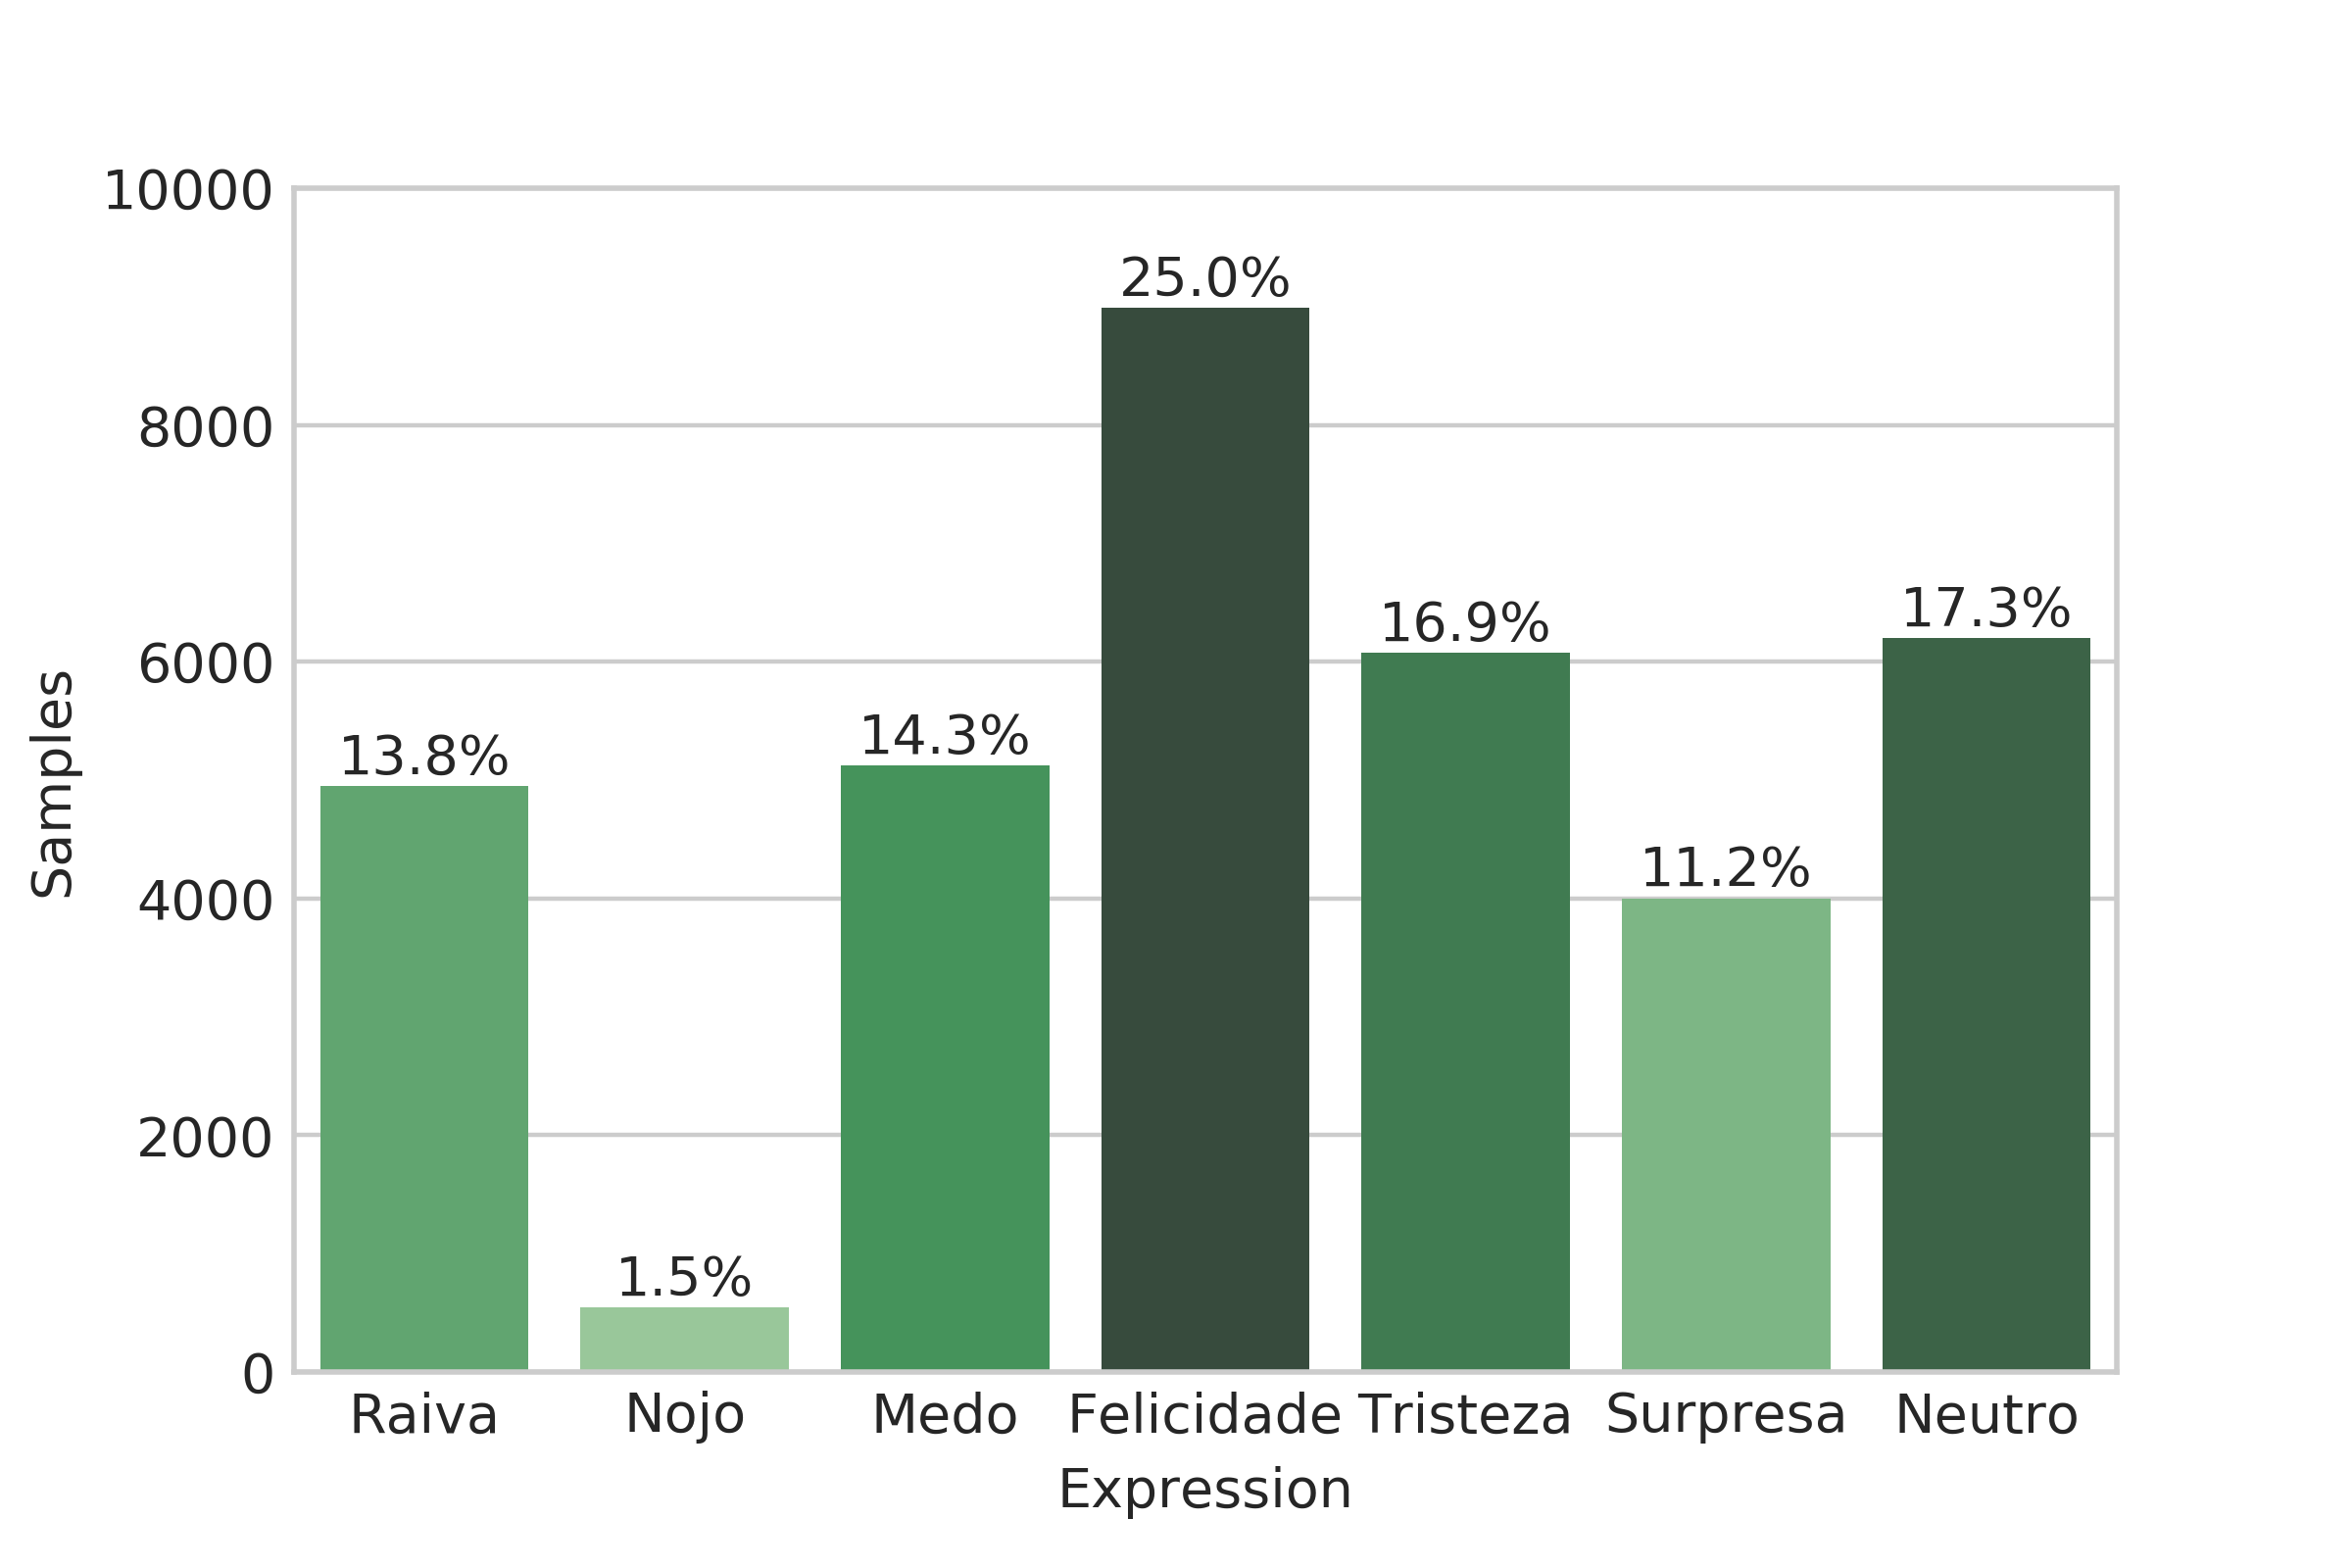
\includegraphics[width=10cm]{images/expression_distribution.png}
\end{figure}
